\documentclass[conference]{IEEEtran}
\IEEEoverridecommandlockouts
\usepackage{cite}
\usepackage{amsmath,amssymb}
\usepackage{graphicx}
\usepackage{url}
\usepackage{booktabs}
\usepackage{enumitem}

\begin{document}

\title{Smart Voice Assistant: A Voice-Driven System for Faster Academic Information Updates in educational institues}

\author{
K.\ Manikandan$^{1}$, R.\ Vishaal$^{2}$, K.\ Santhosh$^{2}$, P.\ Prathas$^{2}$, J.\ Shivaganesh$^{2}$\\
$^{1}$ Assistant Professor, A.V.C.\ College of Engineering, Mayiladuthurai, Tamil Nadu, India\\
$^{2}$ Department of Information Technology, A.V.C.\ College of Engineering, Mayiladuthurai, Tamil Nadu, India
}

\maketitle

\begin{abstract}
This paper presents a smart voice assistant that enables students to access academic information quickly through natural voice interaction. The system combines browser-based speech-to-text and text-to-speech with a web application and a RESTful backend. A lightweight intent handler routes spoken queries to academic services such as timetables, notices, placements, fees, and staff assignments stored in a document database. The design emphasizes usability for students and ease of content updates for faculty and administrators. We describe the system architecture, module responsibilities, implementation choices, and a practical evaluation plan based on response accuracy, latency, and user feedback. The project aims to reduce navigation effort and improve responsiveness of information access.
\end{abstract}

\begin{IEEEkeywords}
voice assistant, academic services, speech recognition, web application, higher education
\end{IEEEkeywords}

\section{Introduction}
In a college environment, timely academic information is critical. Students routinely seek updates about timetables, circulars, fees, and placement activities. Traditional portals require multiple clicks, logins, and manual searches. This process is slow, especially when students are on mobile devices or when information needs to be accessed quickly between classes. Voice-driven interfaces can reduce these barriers by allowing students to ask direct questions and receive immediate spoken responses.

This project develops a smart voice assistant focused on academic information updates. It provides a voice-first experience for students while ensuring that the underlying data remains structured and easy to maintain by faculty or administrative staff. The system is designed to be lightweight, reliable, and deployable in a typical college environment without specialized hardware.

The remainder of this paper covers the problem statement, objectives, system architecture, module design, implementation details, evaluation plan, limitations, and future work. The writing is oriented toward an applied project perspective, emphasizing clear design choices and practical outcomes.

\section{Related Work and Research Gap}
Existing academic chatbots have focused on web-based text interaction and domain-specific guidance. A Dialogflow-based university website chatbot simplifies student queries but remains primarily text-driven and tied to web navigation workflows \cite{b1}. Mental wellness chatbots emphasize counseling and supportive conversation rather than operational academic updates \cite{b2}. Admission and educational guidance assistants prioritize counseling for prospective students, not day-to-day campus services \cite{b3}. Recent work using Llama-3 with retrieval-augmented generation targets broad university support services, but it assumes heavier infrastructure and does not emphasize a lightweight, voice-first interaction loop for routine academic updates \cite{b4,b5}.

The gap identified across these studies is a practical, low-overhead voice assistant that connects directly to institutional records and answers routine academic queries with minimal interaction steps. This paper addresses that gap by implementing a browser-based voice interface, a focused intent handler for predictable academic tasks, and a backend integrated with college data sources.

\section{Problem Statement and Objectives}
\subsection{Problem Statement}
Students need quick access to frequently changing academic information, but existing systems often require manual navigation and repeated searching. Delays in accessing updates can lead to missed deadlines, confusion about schedule changes, and reduced engagement. There is a need for a unified, voice-driven interface that supports immediate responses and integrates seamlessly with academic data.

\subsection{Objectives}
The main objectives of the project are:
\begin{itemize}[leftmargin=*]
\item Provide a voice-based interface for common academic queries.
\item Reduce the time and effort required to access updates.
\item Maintain a modular backend that supports structured data storage.
\item Ensure the system is easy to update and scalable for future features.
\item Preserve clarity and reliability of responses using controlled intent handling.
\end{itemize}

\section{System Overview}
The system follows a simple voice-first interaction flow:
\begin{enumerate}[leftmargin=*]
\item The student speaks a question using the web interface.
\item The browser converts speech to text using built-in speech recognition.
\item The backend maps the query to a specific academic intent.
\item Relevant data is retrieved from the database.
\item A text response is generated and spoken back to the student.
\end{enumerate}

This flow enables fast, hands-free access to information without forcing the student to navigate multiple screens or menus. The architecture is intentionally modular so that individual services can be improved without affecting the overall system.

In practice, the assistant is used in short bursts between classes. The interface is optimized for quick responses rather than long conversations. The response is visible as text and also spoken aloud, which benefits users in hands-free or low-attention settings. The design intentionally favors stable, predictable answers over open-ended chat behavior.

\section{Architecture and Modules}
The overall architecture is shown in Fig.~\ref{fig:architecture}. The system separates client interaction, server-side logic, and data persistence, ensuring maintainability and clear responsibility boundaries.

\begin{figure*}[htbp]
\centerline{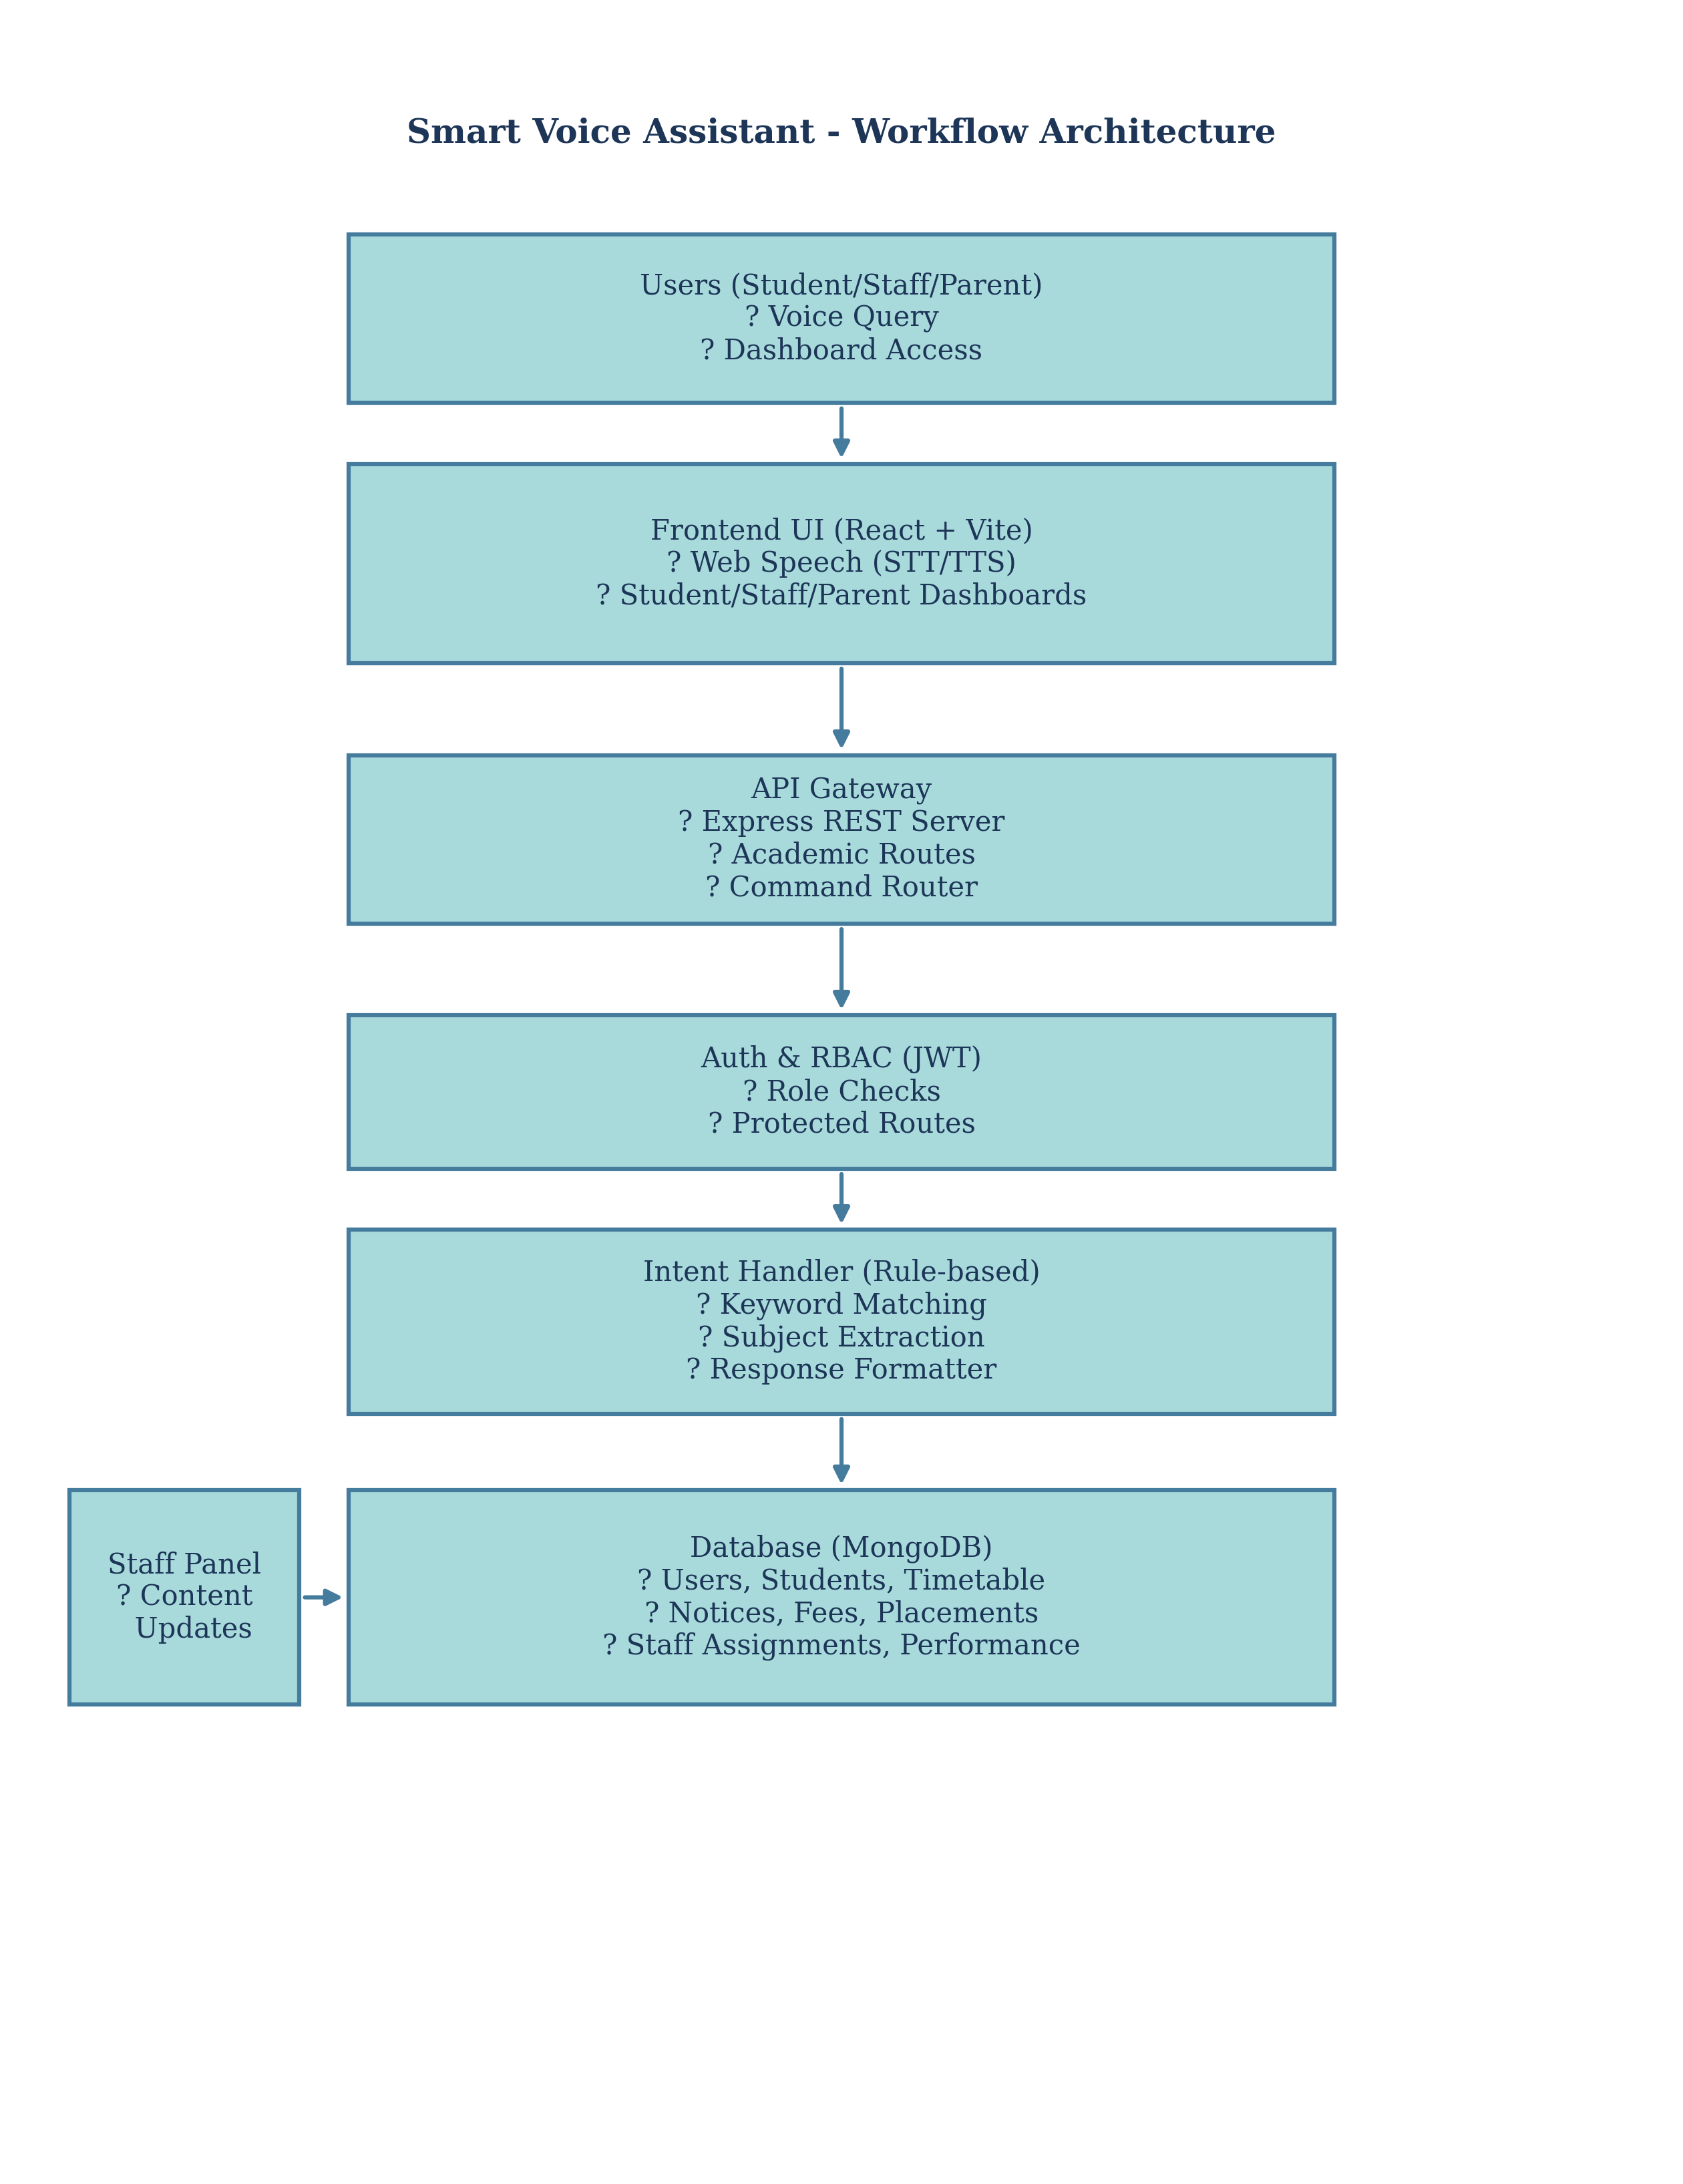
\includegraphics[width=0.90\linewidth]{arch/workflow.png}}
\caption{Vertical workflow architecture of the smart voice assistant.}
\label{fig:architecture}
\end{figure*}

\subsection{Frontend (Voice Interface)}
The frontend is implemented with React and provides a compact voice interface. It uses the browser Web Speech API to capture speech and convert it to text. The interface displays the recognized query, renders the assistant reply, and uses text-to-speech to speak the response. The UI is intentionally minimal to reduce cognitive load and support rapid interactions.

\subsection{Backend Services}
The backend is implemented in Node.js with Express. It exposes REST endpoints for authentication and academic services. A dedicated command endpoint receives recognized text and routes it through the intent handler. The backend also validates requests and formats responses to keep them consistent and user-friendly.

\subsection{Intent Handler}
The intent handler performs lightweight rule-based matching. It identifies keywords, extracts subjects, and maps the query to one of the defined academic services. The rule-based approach is reliable for a narrow academic domain and ensures predictable answers. It also avoids the overhead of training complex models while maintaining responsiveness.

\subsection{Data Layer}
MongoDB stores academic records in structured collections, including users, students, timetable entries, notices, circulars, fees, placements, and staff assignments. The data model is designed for fast retrieval and easy updates by staff. This supports real-time updates as new notices or schedule changes are published.

\subsection{User Roles and Access Control}
The system supports three roles: student, staff, and parent. Staff users can create, edit, and delete academic records. Students are read-only for academic data, while parents can view linked student details and performance. Authentication uses JWT tokens, and role checks are enforced at the API layer to prevent unauthorized access. This separation ensures that sensitive updates remain controlled by authorized staff, while end users receive reliable read access.

\subsection{Data Model Summary}
The academic collections are designed to mirror common college operations. Timetable entries track day, subject, and time. Notices and circulars store titles, content, and dates. Fee records include department, year, total fee, and due date. Placement updates capture company, package, eligibility, and date. Staff assignments map faculty names to subjects and include optional profile metadata such as designation and qualifications. Student performance records track attendance and subject-wise marks for parent access.

\section{Module Description}
Table~\ref{tab:modules} summarizes the major modules and their responsibilities.

\begin{table}[htbp]
\caption{System Modules and Responsibilities}
\label{tab:modules}
\centering
\begin{tabular}{@{}ll@{}}
\toprule
\textbf{Module} & \textbf{Responsibility} \\
\midrule
Voice UI & Capture speech, show replies, speak output \\
API Gateway & Route requests to services and responses \\
Intent Handler & Detect intent and map to services \\
Academic Services & Fetch timetable, notices, fees, placements \\
Database Layer & Store and retrieve academic data \\
\bottomrule
\end{tabular}
\end{table}

Each module is implemented with clear responsibilities to keep maintenance simple. The voice UI captures audio, displays the recognized sentence, and plays the reply using text-to-speech. The API gateway validates requests, enforces authentication, and normalizes responses to keep output consistent. The intent handler maps academic keywords and patterns to services, ensuring predictable routing for queries such as timetables, notices, fees, placements, and staff assignments. The academic services layer encapsulates business logic for each feature and exposes a clear interface to the rest of the system. The database layer holds structured collections to enable fast lookups and reliable updates by staff.

\section{API Endpoints Summary}
Table~\ref{tab:apis} outlines representative endpoints used by the system. The write routes are protected and restricted to staff, while read routes are open to students or parents as appropriate.

\begin{table}[htbp]
\caption{Representative API Endpoints}
\label{tab:apis}
\centering
\begin{tabular}{@{}lll@{}}
\toprule
\textbf{Endpoint} & \textbf{Method} & \textbf{Purpose} \\
\midrule
/api/login/student & POST & Student login (JWT) \\
/api/login/staff & POST & Staff login (JWT) \\
/api/login/parent & POST & Parent login (JWT) \\
/api/timetable & GET & Read timetable entries \\
/api/timetable & POST & Add timetable entry (staff) \\
/api/notices & GET & Read notices \\
/api/notices & POST & Add notice (staff) \\
/api/fees & GET & Read fee details \\
/api/fees & POST & Add fee details (staff) \\
/api/placements & GET & Read placement updates \\
/api/placements & POST & Add placement entry (staff) \\
/api/circulars & GET & Read circulars \\
/api/circulars & POST & Add circular (staff) \\
/api/staff-assignments & GET & Read staff allocations \\
/api/staff-assignments & POST & Add staff allocation (staff) \\
/api/student-performance & POST & Add performance record (staff) \\
/api/parent/students & GET & Parent-linked students \\
/api/parent/performance & GET & Parent performance view \\
/api/command & POST & Voice command intent handler \\
\bottomrule
\end{tabular}
\end{table}

\section{Methodology}
The methodology follows a stepwise pipeline, similar to a classroom workflow, to ensure accurate interpretation and response delivery.

\subsection{Step 1: Voice Input}
The user speaks a query through a microphone-enabled device. The interface records the audio stream and initiates processing without requiring any typing. This step emphasizes natural interaction and reduces friction for students accessing information between classes.

\subsection{Step 2: Speech-to-Text Conversion}
The captured audio is converted into text using the browser speech recognition engine. The system handles variations in accent and speaking speed. The recognized text is displayed to the user to provide transparency and confirm the captured query.

\subsection{Step 3: Intent and Keyword Analysis}
The text is passed to the intent handler, which detects the query category using controlled keyword rules. The handler extracts the required subject, department, or date reference from the sentence and maps the request to the correct academic service. This targeted approach keeps responses stable and avoids ambiguity.

The command handler also normalizes text by lowering case, removing extra whitespace, and checking for keyword variants (for example, ``time table'' vs.\ ``timetable''). This improves robustness without introducing heavy NLP processing.

\subsection{Step 4: Data Retrieval}
The academic service constructs a database query and retrieves relevant records. Data is fetched from structured collections that store timetables, notices, fee details, placement drives, and staff information. Only the data needed for the response is returned, keeping latency low.

\subsection{Step 5: Response Generation and Speech Output}
The backend formats the answer in clear natural language. The frontend displays the response and uses text-to-speech to read it aloud. This completes the interaction cycle and ensures that users can access results without needing to read a screen.

\section{Queries Supported}
The assistant is designed around common academic questions. Typical queries include:
\begin{itemize}[leftmargin=*]
\item ``What is my timetable today?''
\item ``Show the latest notice.''
\item ``When is the next exam for Database Systems?''
\item ``What is my attendance percentage?''
\item ``Tell me the fee due date.''
\item ``Which company is visiting for placements this week?''
\item ``Who is the staff in charge of Operating Systems?''
\end{itemize}

The voice assistant is optimized for short, direct questions. Responses are returned in a compact natural-language format so that the spoken reply remains concise and easy to understand. This design avoids long passages that might be difficult to follow in a spoken-only interaction.

\section{Implementation Details}
The system uses the following stack:
\begin{itemize}[leftmargin=*]
\item \textbf{Frontend:} React with Vite for a fast, modular web interface.
\item \textbf{Speech:} Web Speech API for browser-based speech recognition and text-to-speech.
\item \textbf{Backend:} Node.js with Express to expose REST endpoints and route commands.
\item \textbf{Database:} MongoDB with Mongoose to model academic collections.
\item \textbf{Security:} JWT for session management and bcrypt for password hashing.
\end{itemize}

Speech input is posted to the backend command endpoint. The server checks for keywords (such as ``timetable'', ``notice'', ``placement'', or ``fees''), determines the most likely intent, and returns a natural-language response. The client renders the reply text and uses text-to-speech to speak the answer. This pipeline provides an end-to-end response that is both visible and audible.

The frontend provides separate dashboards for students, staff, and parents. Staff can update records for timetables, notices, circulars, fees, and placements. Parents can view assigned staff, student records, and monthly performance. Students receive read-only academic updates and can interact through voice queries. This separation aligns with real-world academic roles and reduces the chance of accidental edits by end users.

\section{Design Choices and Rationale}
Several design choices were made to ensure that the system remains practical and efficient:
\begin{itemize}[leftmargin=*]
\item \textbf{Rule-based intent handling:} Focused academic queries benefit from simple keyword rules, which produce consistent results and reduce computational overhead.
\item \textbf{Browser-based speech recognition:} Using the Web Speech API avoids external dependencies and keeps the client lightweight.
\item \textbf{Document database:} MongoDB supports flexible academic data models and rapid updates.
\item \textbf{Modular service endpoints:} Individual services (timetable, notices, fees) can be expanded independently.
\end{itemize}

This approach favors reliability and speed while keeping the system easy to maintain and extend.

\section{User Interface Design}
The student dashboard emphasizes quick access to voice input and concise result summaries. Cards display the most recent academic records so that students can verify updates without navigating multiple pages. The staff panel provides structured forms for each academic service to reduce entry errors and simplify updates. Parent views focus on staff allocations and student performance, emphasizing clarity and readability. Across dashboards, the layout minimizes visual clutter and supports common device sizes used on campus.

\section{Security and Privacy Considerations}
Authentication uses JWT tokens with role checks enforced by the backend. Sensitive routes require staff or parent roles, and responses are normalized to avoid exposing internal details. Passwords are hashed using bcrypt. The design assumes that the institution manages user credentials and that access policies align with internal privacy norms. While the system does not store audio recordings, it handles student-related data that should be protected according to campus policy.

\section{Performance Considerations}
The backend relies on direct MongoDB queries for fast read access and uses indexed fields for common lookups where applicable. Voice requests are handled with lightweight rule checks, reducing processing time. The response format is intentionally concise so that text-to-speech remains clear and does not add excessive latency. These choices favor predictable performance under typical campus network conditions.

\section{Testing and Validation}
The backend includes automated tests that verify role-based access control and CRUD behavior for academic services. Tests check that staff users can create and update records, while students and parents receive appropriate access restrictions. API responses are validated for expected status codes, and common error cases (missing tokens, invalid permissions) are included. This test coverage provides confidence that the system behaves correctly under typical usage and helps prevent regressions.

\section{Deployment and Configuration}
The system is designed for standard deployment on a local server or campus network. The backend runs on Node.js with a configurable MongoDB connection string. The frontend is bundled with Vite and can be hosted as static assets. Environment variables are used for sensitive settings such as JWT secrets. This configuration keeps setup simple for small institutions while remaining compatible with larger deployments.

\section{Use Cases}
The following use cases capture typical interactions:
\begin{enumerate}[leftmargin=*]
\item \textbf{Timetable Query:} A student asks for today’s timetable, and the assistant responds with class times and subjects.
\item \textbf{Notice Update:} A student requests the latest notice; the system fetches the most recent entry and reads it aloud.
\item \textbf{Fee Information:} A student asks about fees and due dates; the assistant returns the total fee and deadline.
\item \textbf{Placement Update:} A student asks about placement drives and receives the latest company and eligibility details.
\item \textbf{Staff Assignment:} A student asks who handles a subject; the assistant replies with the assigned faculty.
\end{enumerate}

\section{Evaluation Plan}
Since full-scale deployment data is not yet available, the evaluation plan focuses on practical metrics that can be measured with a limited pilot:
\begin{itemize}[leftmargin=*]
\item \textbf{Intent Accuracy:} Measure how often queries are mapped to the correct service using a manual test set of typical student queries.
\item \textbf{Latency:} Measure time from speech end to spoken reply on common hardware and network conditions.
\item \textbf{User Satisfaction:} Collect feedback using a short Likert-scale survey focusing on usefulness, clarity, and speed.
\end{itemize}

These metrics provide actionable feedback while keeping evaluation practical for a college project.

Additional qualitative feedback can be collected from staff to assess whether the management dashboards reduce update effort compared to traditional notice-board workflows. This perspective helps measure the system's operational value, not just student-facing usability.

\section{Discussion}
The voice-first interaction model reduces the effort required to retrieve academic information. The rule-based intent handler offers predictable behavior, which is beneficial for academic use cases where clarity and reliability matter more than open-ended conversation. The modular architecture supports incremental improvements without disrupting existing services.

The system is designed to be maintainable. Academic data can be updated through the backend without changing the frontend. This separation is important because institutional data changes frequently, while the student-facing interface can remain stable.

\section{Limitations}
\begin{itemize}[leftmargin=*]
\item Rule-based intent matching may not handle complex, ambiguous queries.
\item Browser speech recognition depends on device quality and network stability.
\item The current evaluation plan relies on pilot testing rather than large-scale deployment.
\end{itemize}

\section{Future Work}
Planned improvements include:
\begin{itemize}[leftmargin=*]
\item A richer NLP model for flexible phrasing.
\item Analytics dashboard for staff to view usage trends.
\item Multilingual support for wider accessibility.
\item Integration with college ERP for real-time updates.
\item Push notifications for critical announcements.
\end{itemize}

\section{Conclusion}
This paper presented a smart colleg assistant tailored for academic information updates in colleges. The system provides a fast and natural interface for students while maintaining a clean backend architecture for administrators. The solution demonstrates how voice interfaces can improve accessibility and efficiency in higher education settings, and it offers a foundation for future enhancements such as multilingual support and analytics.

\section*{Acknowledgment}
The authors thank Dr.\ K.\ Manikandan (Assistant Professor), A.V.C.\ College of Engineering, for his guidance and support. Dr.\ K.\ Manikandan holds M.C.A., M.Phil., M.Tech., and Ph.D. degrees.

\begin{thebibliography}{00}
\bibitem{b1} Author(s), ``Multimodal AI for Romanian University Support: An LLM, RAG and Voice Approach,'' in \emph{Proceedings of the [Conference Name]}, [City, Country], 2025, pp.~[xx--xx].
\bibitem{b2} Author(s), ``Chatbot for Student Descipline Handbook-Related Queries: A RAG-Based LLM Using Llama-3 Approach,'' in \emph{Proceedings of the [Conference Name]}, [City, Country], 2025, pp.~[xx--xx].
\bibitem{b3} Author(s), ``Simplifying Student Queries: A Dialogflow-Based Conversational Chatbot for University Websites,'' in \emph{Proceedings of the [Conference Name]}, [City, Country], 2025, pp.~[xx--xx].
\bibitem{b4} Author(s), ``An Enhanced Chatbot for University Admission and Educational Guidance,'' in \emph{Proceedings of the [Conference Name]}, [City, Country], 2025, pp.~[xx--xx].
\bibitem{b6} Author(s), ``Mental Wellness ChatBot for Students Using NLP,'' in \emph{Proceedings of the [Conference Name]}, [City, Country], 2025, pp.~[xx--xx].
\bibitem{b7} Author(s), ``Chatbots in Academia: A Retrieval-Augmented Generation Approach for Improved Efficient Information Access,'' in \emph{Proceedings of the [Conference Name]}, [City, Country], 2024, pp.~[xx--xx].
\bibitem{b8} Author(s), ``AI-Driven Academic Assistant: Leveraging Llama-3 and RAG for Enhanced University Support Services,'' in \emph{Proceedings of the [Conference Name]}, [City, Country], 2024, pp.~[xx--xx].
\bibitem{b10} Author(s), ``VoiceTalk: A No-Code Approach for Creating Voice-Controlled Smart Home Applications,'' in \emph{Proceedings of the [Conference Name]}, [City, Country], 2025, pp.~[xx--xx].
\end{thebibliography}

\end{document}

